% !TEX root = /home/benedict/Documents/Studium/Studienarbeit/Studienarbeit_Graphen_Metriken_Aehnlichkeit/Arbeit/T3101_Studienarbeit_GraphenMetriken_Weichselbaum_TINF2018.tex

\documentclass[a4paper,12pt,ngerman,chapterprefix=false,listof=totoc,bibliography=totoc]{scrreprt}

\usepackage[a4paper,left=2.5cm, right=2.5cm, top=2cm, bottom=2.5cm]{geometry}
\usepackage[ngerman, english]{babel}
\usepackage{blindtext}
\usepackage{helvet}
\usepackage{subcaption}
\usepackage[utf8]{inputenc}
\renewcommand{\familydefault}{\sfdefault}

\usepackage{microtype}
\usepackage{graphicx}
\usepackage{wrapfig}
\usepackage{enumitem}
\usepackage{amsmath}
\usepackage{index}
\usepackage{csquotes}
\usepackage[onehalfspacing]{setspace}
\usepackage{listings}
\usepackage{changepage}
\usepackage{acronym}
\usepackage{listings}
\usepackage{abstract}
\usepackage{scrhack}
\usepackage{booktabs}
\usepackage{pdflscape}
\usepackage{hyperref}
\usepackage{svg}
\usepackage{mathtools}
\hypersetup{
    colorlinks,
    citecolor=black,
    filecolor=black,
    linkcolor=black,
    urlcolor=black
}
\usepackage[bottom]{footmisc}

% Biblatex includes
\usepackage[style=alphabetic,backend=biber]{biblatex}
\addbibresource{literatur.bib}

\usepackage{listings}
\usepackage{xcolor}

\DeclarePairedDelimiter{\ceil}{\lceil}{\rceil}

\definecolor{codegreen}{rgb}{0,0.6,0}
\definecolor{codegray}{rgb}{0.5,0.5,0.5}
\definecolor{codepurple}{rgb}{0.58,0,0.82}
\definecolor{backcolour}{rgb}{0.95,0.95,0.92}

\lstdefinestyle{mystyle}{
    backgroundcolor=\color{backcolour},   
    commentstyle=\color{codegreen},
    keywordstyle=\color{magenta},
    numberstyle=\tiny\color{codegray},
    stringstyle=\color{codepurple},
    basicstyle=\ttfamily\footnotesize,
    breakatwhitespace=false,         
    breaklines=true,                 
    captionpos=b,                    
    keepspaces=true,                 
    numbers=left,                    
    numbersep=5pt,                  
    showspaces=false,                
    showstringspaces=false,
    showtabs=false,                  
    tabsize=2
}

\lstset{style=mystyle}

% Custom environments
\newenvironment{myitemize}{\begin{itemize}\itemsep -4pt}{\end{itemize}}
\newenvironment{myenumerate}{\begin{enumerate}\itemsep -4pt}{\end{enumerate}}
\newenvironment{myalphaenum}{\begin{enumerate}[label={\alph*)}]\itemsep -4pt}{\end{enumerate}}

% Custom commands
\newcommand{\absatz}{{\vspace{5mm}\newline}}
\newcommand{\zitat}[2]{
	\begin{quote}
		\textit{#1} \cite{#2}
	\end{quote}
}	
	
\newcommand{\geintrag}[2]{
	\textbf{#1}\begin{adjustwidth}{.5cm}{0cm}#2
	\end{adjustwidth}\vspace{3.5mm}
}
\newcommand{\singleenum}[2]{
	\begin{myenumerate}
		\setcounter{enumi}{#1}
		\item #2
	\end{myenumerate}
}

\newcommand{\specialcell}[2][l]{%
  \begin{tabular}[#1]{@{}l@{}}#2\end{tabular}}

\newcommand{\metric}[2]{
	\textbf{#1}
	\begin{adjustwidth}{.5cm}{0cm}
		%\begin{tabular}{p{28mm} p{115mm}}
		%	Definition: & \specialcell{#2} \\
		%	Komplexität: & \specialcell{#3}
		%\end{tabular}
		#2
	\end{adjustwidth}\hrulefill\\\vspace{2mm}
}

% Settings for bibliography from BibLaTeX
\setcounter{biburllcpenalty}{7000}
\setcounter{biburlucpenalty}{8000}

\AfterTOCHead{\thispagestyle{empty}}

\begin{document}
\title{\Large{Untersuchung, Implementierungen und Bewertung von Graph-Metriken
}}
\author{Benedict Martin Weichselbaum}
\date{\today}
\selectlanguage{ngerman}
\begin{titlepage}
	\centering\hspace{8mm}
	\begin{figure}
		\centering
			
\includegraphics[scale=1.3]{./Abbildungen/dhbwlogo.png}
	\end{figure}
	
	\vspace{5mm}	
	{\fontsize{26}{40}\selectfont
	Untersuchung, Implementierungen und Bewertung von Graph-Metriken
	}
	\\
	\vspace{2cm}
	\textbf{\Large{Studienarbeit}} \par
	\vspace{1cm}
	im Studiengang Informatik \par
	\vspace{0.3cm}
	an der Dualen Hochschule Baden-Württemberg Stuttgart, Campus Horb am Neckar \par
	\vspace{1.2cm}
	von \par
	\vspace{0.5cm}
	\textbf{\large{Benedict Weichselbaum}} \par
	\vspace{1.5cm}
	{\today}\par
	\vfill
	\begin{table}[ht]
		\hspace{1,5cm}
		\begin{tabular}{p{7cm}p{7cm}}
			\textbf{Bearbeitungszeitraum} & 28.09.2020 - 31.05.2021\\
			\textbf{Matrikelnummer, Kurs} & 6275457, TINF2018\\
			\textbf{Betreuer \& Gutachter} & Prof. Dr. ing. Olaf Herden\\
		\end{tabular}
	\end{table}
\end{titlepage}

\section*{Erklärung}
\thispagestyle{empty}
Ich versichere hiermit, dass ich meine Studienarbeit mit dem Thema \textit{Graphen: Metriken und Ähnlichkeit} selbstständig verfasst und keine anderen als die angegebenen Quellen und Hilfsmittel benutzt habe.
\newline
Ich versichere zudem, dass die eingereichte elektronische Fassung mit der gedruckten Fassung übereinstimmt.\vspace{1.6cm}\newline
{Nürnberg, \today\vspace{1.2cm}\par\vspace{1.5cm}}
{\noindent\rule{6cm}{.4pt}\newline Benedict Martin Weichselbaum}

\selectlanguage{english}
\begin{abstract}
	
\end{abstract}

\selectlanguage{ngerman}
\setcounter{tocdepth}{3}

{\tableofcontents \thispagestyle{empty}}


\listoffigures\thispagestyle{plain}
\pagenumbering{Roman}
\setcounter{page}{1}

\listoftables\thispagestyle{plain}

\chapter*{Abkürzungsverzeichnis}
\addcontentsline{toc}{chapter}{Abkürzungsverzeichnis}
\begin{acronym}

\end{acronym}


\chapter{Einleitung}
\pagenumbering{arabic}
\setcounter{page}{1}
\section{Motivation für die Studienarbeit}{
Graphen sind einer der wichtigsten Datenstrukturen der Informatik. Warum kann man das sagen? In seinem Buch "`Algorithmische Graphentheorie"' nennt Volker Turau, Professor an der Universität Hamburg-Harburg, den Grund dafür: 
\zitat{Graphen sind die in der Informatik am häufigsten verwendete Abstraktion. Jedes System, welches aus diskreten Zuständen oder Objekten und Beziehungen zwischen diesen besteht, kann als Graph modelliert werden.}{turau_algorithmische_2004}
Diese netzartigen Strukturen können dabei die verschiedensten Konstrukte repräsentieren. Dazu zählen Straßennetze, Computernetzwerke, elektrische Schaltungen aber auch zum Beispiel chemische Moleküle. \cite{tittmann_graphentheorie_2019}

Um Graphen zu beschreiben und zu charakterisieren, haben sich über die Zeit zahlreiche Metriken, bzw. Eigenschaften für diese herausgebildet ("`graph properties"' \cite{lovasz_large_2012}). Das heißt, einem Graphen können gewisse Kennzahlen zugeordnet werden, die ihn auszeichnen. Auch diese Metriken sind, wie die Graphen selbst, oft praktisch anwendbar. Zum Beispiel in der Untersuchung von Netzwerken \cite{ellens_graph_2013}.

Diese Studienarbeit soll nun diese Metriken genauer untersuchen. Hierbei ist es zunächst wichtig die verschiedenste Metriken vorzustellen und zu erläutern. Dabei ist es auch wichtig herauszufinden, wie verbreitet diese Metriken sind und inwieweit die jeweiligen Kennzahlen zu bewerten sind. Des Weiteren soll auf Basis der Metriken auch der Begriff der Ähnlichkeit von Graphen aufgegriffen werden.

Neben einer theoretischen Betrachtung der Graphmetriken soll auch eine Implementierung stattfinden. Es ist dabei das Ziel, mithilfe von Graphdatenbanken die jeweiligen Metriken umzusetzen und diese miteinander zu Vergleichen.

In einem Weiteren Teil ist außerdem noch darauf einzugehen, welche Anwendung die gezeigten Metriken haben, um den praktischen Nutzen der Thematik aufzuzeigen.
}
\section{Fragestellungen}
{
Auf Basis dieser Motivation können nun auch die konkreten Fragestellungen formuliert werden, die diese Arbeit betrachten soll. Insgesamt sollen vier wissenschaftliche Fragen beantwortet werden.

\singleenum{0}{Welche Graph-Metriken gibt es und wie sind diese definiert und zu kategorisieren?}

Hierzu gehört, wie bereits erwähnt die Vorstellung der einzelnen Metriken, aber auch eine Kategorisierung in Rubriken, um Metriken besser voneinander abzugrenzen, da diverse Metriken höchst unterschiedliche Aussagen über einen Graphen treffen. Es wird auch darauf eingegangen welche Motivation hinter den jeweiligen Metriken steht.  Bei der Beantwortung dieser Frage soll außerdem auch darauf eingegangen werden, inwieweit die beschriebene Metrik in bestimmten Mathematikbibliotheken wie "`Sage Math"' oder "`Wolfram"' vorkommen.

\singleenum{1}{Wie sind die vorgestellten Metriken zu bewerten?}

Bei dieser Frage soll es vor allem darum gehen, die vorgestellten Metriken dahingehend zu bewerten, wie "`schwer"' es ist, sie zu ermitteln. Außerdem wird bei der Bewertung auch auf die Verbreitung eingegangen. Speziell soll erwähnt werden, ob die jeweilige Metrik in bekannten Mathematikbibliotheken vertreten ist oder nicht.

\singleenum{2}{Was beschreibt der Ähnlichkeitsbegriff bei Graphen?}

Basierend auf Graph-Metriken lässt sich auch ermitteln, ob zwei Graphen Ähnlichkeiten aufweißen \cite{wills_metrics_2019}. Auch auf diesen Aspekt soll die Arbeit bezug nehmen und dabei ein Anwendungs-Beispiel konstruieren.

\singleenum{3}{Wie können die vorgestellten Metriken in Graphdatenbanken verwendet werden, bzw. implementiert werden?}

Auf die theoretische Betrachtung der Graph-Metriken folgt dann ein praktischer Teil, der behandeln soll, wie sich die Metriken in bekannten Graphdatenbanken umsetzen lassen, bzw. umgesetzt wurden. Dabei ist es wichtig herauszufinden welche Graphkennzahlen bereits teil der Graphdatenbank-Lösungen sind, bzw. welche Metriken selbst umgesetzt werden müssen.

\singleenum{4}{Wie sind die jeweiligen Implementierungen zwischen und innerhalb der Graphdatenbanken zu bewerten?}

Folgend auf die Implementierung, ist es noch wichtig zu verstehen, wie diese Umsetzungen zu betrachten sind. Dabei wird vor allem ein Fokus auf das Thema Performance und Skalierung gelegt.

\singleenum{5}{Welche Anwendungen gibt es für Graph-Metriken und den Vergleich von Graphen (Ähnlichkeit)?}

Als letztes soll sich die Studienarbeit mit praktischen Beispielen beschäftigen. Es ist dabei wichtig zu verstehen, welchen konkreten Nutzen die gezeigten Kennzahlen für Graphen in modernen Anwendungsszenarien haben.
}
\chapter{Graph-Metriken}
{
Dieser erste Teil der Arbeit wird sich nun ausführlich mit einer weiten Reihe an Graph-Metriken beschäftigen. Hierbei sollen die ersten zwei Fragestellungen der Arbeit genau beantwortet werden. Zur jeweiligen Vorstellung einer Graph-Metrik sollen dabei die folgengen Punkte erläutert werden:
\begin{myitemize}
	\item Was drückt die Metrik aus (Definition)?
	\item Wie ist die Metrik im Bezug auf den Rechenaufwand zu bewerten?
	\item Inwieweit ist die Metrik verbreitet? Zum Beispiel in der Literatur oder in Mathematikbibliotheken.
	\item Was ist eine konkrete Motivation bzw. Anwendung für die Metrik, falls diese auszumachen ist?
\end{myitemize}
Es ist noch zu erwähnen, dass alle im folgenden vorgestellten Metriken über die einzelnen Sektionen der Arbeit in ihre Kategorien eingeteilt sind. Als Synonym für Metrik werden innerhalb dieser Arbeit die Begriffe Kennzahl und Invariante gebraucht. Eine Invariante ist dabei speziell eine Funktion, die zwei isomorphen Graphen den gleichen Wert zuordnet. Dies ist gleichwertig mit dem Begriff Metrik, da eine Metrik auch einen Graphen auf eine Zahl bzw. einen Wert abbildet. \cite{diestel_graphentheorie_2000}

Darüber hinaus ist noch eine grundsätzliche Notationen während der Arbeit zu klären: Ein \textbf{Graph G} ist ein Paar bestehend aus \textbf{Knoten V} und \textbf{Kanten E}.
\begin{align*}
	G = (V, E),\ wobei\ E \subseteq V \times V
\end{align*}
Für V können wir auch V(G) schreiben, für E auch E(G). \cite{diestel_graphentheorie_2000} V ist dabei Englisch und bedeutet "`Vertices"', E steht für "`Edges"'. Wenn es um die Datenstrukturen von Graphen geht, kommen im Rahmen dieser Arbeit hauptsächlich Adjazenzmatrizen und Adjazenzlisten zum Einsatz. Allerdings können bei Bedarf auch Inzidenzen (Beziehung zwischen Knoten und Kanten) im Graphen eine Rolle spielen, wie Inzidenzmatrizen und Inzidenzlisten. \cite{knebl_algorithmen_2019,diestel_graphentheorie_2000} Zudem wird bei der Betrachtung meist auf ungerichtete, simple Graphen Bezug genommen.
}
\section{Grundlegende Metriken}
{
Ein einem ersten Teil sollen grundlegende Graph-Kennzahlen vorgestellt werden. Diese beschreiben einen Graphen auf rudimentäre Art und Weise und zeigen die am einfachsten zu berechnenden Eigenschaften des Graphen.
}
\subsubsection*{Ordnung und Größe eines Graphen}
{
Die Frage danach, wie viele Knoten ein Graph hat lässt sich mit der \textbf{"`Ordnung"'} eines Graphen beantworten. Die "Ordnung" beschreibt dabei einfach die Anzahl der Elemente in der Menge V. Man schreibt: \(\vert V\vert\ oder\ \vert V(G)\vert\ oder\ auch\ \vert G\vert\). \cite{diestel_graphentheorie_2000} Diese Eigenschaft ist essentiell zur allgemeinen Beschreibung und z.B. graphischen Darstellung eines Graphen. Sie lässt sich dabei in sämtlichen mathematischen Bibliotheken finden, wie SageMath, Matlab und Wolfram \cite{sagemath_graph_2020,matlab_directed_2020,wolfram_graph_2020}. Die Komplexität zur Erfassung der Metrik gestaltet sich dabei äußerst einfach. Bei einer Adjazenzmatrix lässt sich die Anzahl der Knoten dadurch herausfinden, wie "`lang"' eine Dimension des zweidimensionalen Arrays bzw. der zweidimensionalen Liste. Dies kann man je nach Implementierung der jeweiligen Datenstruktur in einer Komplexität von \(O(n)\) oder \(O(1)\) herausfinden.

Eine weitere grundlegende Kennzahl von Graphen ist dessen \textbf{"`Größe"'}. Die Größe beschreibt dabei die Anzahl der Kanten, die im Graphen vorkommen, also die Anzahl der Elemente in der Menge E. Man schreibt analog zur Größe des Graphen: \(\vert E\vert\ oder\ \vert E(G)\vert\ oder\ auch\ \vert\vert G \vert\vert\). \cite{balakrishnan_schaums_1997,diestel_graphentheorie_2000} Auch diese Metrik ist weit verbreitet. So lässt sie sich in vielen Büchern zur Graphentheorie finden, aber auch in den genannten Mathematikbibliotheken \cite{sagemath_graph_2020,matlab_directed_2020,wolfram_graph_2020}. Die Anzahl der Kanten innerhalb eines Graphen herauszufinden, erweist sich nicht ganz so trivial wie das Herausfinden der Ordnung. Ist ein Graph nicht gerichtet, d.h. seine Kanten haben keine feste Richtung \cite{diestel_graphentheorie_2000} so ist seine Adjazenzmatrix symmetrisch. Man kann also zählen wie viele Einträge es innerhalb der Matrix auf der Hauptdiagonalen und einer der Hälften gibt. Das ergäbe immer \(\frac{1}{2}n^2\) Schritte, wenn \(n\) die Ordnung des Graphen ist. Die Komplexität beträge also \(O(n^2)\). Bei der Darstellung durch eine Inzidenzliste wäre das anders. Hier könnte einfach die Größe der Liste gesucht werden und man wüsste die Größe des Graphen. Die Komplexität wäre hier, wie schon erwähnt, je nach Implementierung \(O(n)\) oder \(O(1)\).
}
\subsubsection*{Der Grad eines Knotens}
{
Während die zwei ersten vorgestellten Metriken vor allem den Graphen als ganzes beschreiben, ist es auch noch wichtig zu wissen, was einen einzelnen Knoten auszeichnet, um einen Graphen besser zu beschreiben. Hierzu gibt es die grundlegende Metrik des \textbf{Grad} eines Knotens. Der Grad eines Knotens beschreibt die Anzahl der mit einem Knoten inzidenten Kanten \cite{diestel_graphentheorie_2000}. D.h. es drückt aus, wie viele Kanten mit einem Knoten verbunden sind. Man kann dies z.B. durch eine Funktion ausdrücken, die einen Knoten v auf eine natürliche Zahl abbildet: \(d(v)\).

Auf Basis dieser Metrik lässt sich auch andere verwandte Metriken ableiten. Hierzu gehört der \textbf{"`Minimalgrad"'} und der \textbf{"`Maximalgrad"'}. Der Minimalgrad ist der kleinste Knoten-Grad eines Graphen G: \(\delta (G):=min\{d(v)\ \vert\ v\ \in\ V(G)\}\). Parallel dazu ist der Maximalgrad der größte Knoten-Grad eines Graphen G: \(\Delta (G)\ :=\ max\{d(v)\ \vert\ v\ \in\ V(G)\}\). Darüber hinaus kann man noch den \textbf{"`Durchschnittsgrad"'} eines Graphen bestimmen. Dieser bildet den Durchschnitt aller Knotengrade ab: \(d(G):=(\sum_{v\in V(G)}d(v))/\vert V\vert\). \cite{diestel_graphentheorie_2000}

Des Weiteren gibt es bei der Betrachtung eines gerichteten Graphen zusätzliche Abwandlungen der Metrik. Da hier die Kanten immer zu einem Knoten gerichtet sind unterscheidet man speziell zwischen dem \textbf{"`Eingangsgrad"'} und dem \textbf{"`Ausgangsgrad"'}. Der Eingangsgrad eines Knoten beschreibt dabei die Anzahl der Kanten, die auf einen Knoten "`zeigen"'. Der Ausgangsgrad zeigt wie viele Kanten von einem Knoten "`weggehen"'. \cite{balakrishnan_schaums_1997}

Auch der Grad eines Knotens und die meisten seiner verwandten Metriken sind weit verbreitet. So sind der allgemeine Grad, der Eingangsgrad, der Ausgangsgrad in allen drei betrachteten Mathematikbibliotheken vorhanden. SageMath unterstützt sogar nativ die Metrik "`Durchschnittsgrad"'. \cite{sagemath_graph_2020,matlab_directed_2020,wolfram_graph_2020}

Die Berechnung eines Grades über eine Adjazenzmatrix oder eine Adjazenzliste ist in linearer Zeit lösbar (\(O(n)\)). Bei der Adjazenzmatrix muss einfach nur die jeweilige Reihe des zugehörigen Knotens durchlaufen werden und gezählt werden, wie häufig ein Eintrag für eine Kante enthalten. Mit Hilfe der Adjazenzliste kann einfach die Größe der Liste als Grad genommen werden, die dem Knoten zugehörig ist.
}
\subsubsection*{Anzahl der Zusammenhangskomponenten}
{
Eine weitere Variante einen Graphen grundlegend zu beschreiben, besteht darin seine Zusammenhangskomponenten zu zählen. Hierfür ist es zunächst wichtig zu verstehen, was Zusammenhang bei Graphen bedeutet.

Ein Graph gilt dann als zusammenhängend, wenn gilt: \(\forall a, b(a\in V \land b\in V \land a\neq b \implies Weg\_existiert(a, b))\). Anschaulich bedeutet das, dass es zwischen zwei beliebigen Knoten immer einen Weg geben muss, der die beiden Knoten miteinander verbindet. Graphisch erscheint ein zusammenhängender Graph so, dass sich keine verschiedenen, klar voneinander trennbaren Komponenten erkennen lassen. Diese einzelnen Komponenten oder Partitionen eines nicht-zusammenhängenden Graphen werden "`Zusammenhangskomponenten"' genannt. Innerhalb der Zusammenhangskomponenten gilt natürlich wieder die Eigenschaft des Zusammenhangs. \cite{diestel_graphentheorie_2000}

Die Anzahl der Zusammenhangskomponenten gibt nun an, wie viele Komponenten innerhalb eines Graphen vorhanden sind. Die Metrik ist sowohl in MatLab als auch in SageMath vertreten \cite{sagemath_graph_2020,matlab_graph_2020}. Zur Ermittlung der Anzahl wird sich eines einfachen Algorithmus bedient, der die Tiefen- oder Breitensuche nutzt, die jeweils jeden Knoten als "`besucht"' markiert, den sie traversiert. Folgender Pseudocode beschreibt diesen Algorithmus:
\begin{lstlisting}
	Integer zaehleKomponenten (graph)
		int komponentenanzahl = 0
		for (knoten in graph)
			if (knoten ist nicht besucht)
				tiefen_oder_breitensuche(graph, knoten)
			komponentenanzahl++
		return komponentenanzahl
\end{lstlisting}
Da der Algorithmus von einem der Suchalgorithmen abhängig ist, bestimmt dieser die Komplexität zur Ermittlung der Kennzahl. Jeder Knoten wird genau einmal in dieser Prozedur besucht. Zudem wird über alle Knoten in der äußeren Zählschleife iteriert. Es ergibt sich dadurch eine Komplexität von \(O(\vert V\vert +\vert E\vert)\).
}
\section{Distanzmetriken}
{
Innerhalb der Graphentheorie gibt es den Begriff des Wegs. Ein Weg beschreibt dabei einen Graphen, der Knoten in einer Reihe hinterander Verbindet. Somit hat der Anfangs- und End-Knoten den Grad 1 und alle "`mittleren"' Knoten den Grad 2. Meist sucht man aber einen bestimmten Weg innerhalb eines bestehenden Graphen. Der Weg ist hier dann ein Teilgraph des ursprünglichen Graphen. Anschaulicher lässt sich ein Weg also als eine Folge von Kanten beschreiben, in der kein Knoten zweimal besucht wird. Die Länge eines Weges ist dabei die Anzahl der Kanten, die in einem Weg vorhanden sind. \cite{diestel_graphentheorie_2000} Auf Basis des Weges und seiner Längen-Eigenschaft lassen sich nun eine Reihe von Metriken definiert werden.
\subsubsection*{Abstand/Distanz}
{
Der "`Abstand"' ist eine Metrik, die auf Basis von zwei Knoten innerhalb eines Graphen definiert wird. Sie beschreibt die Länge des kürzesten Weges zwischen den zwei Knoten, von denen man den Abstand wissen will. Aufgeschrieben werden kann die Metrik mittels einer Funktion, die für den Graph G zwei Knoten x und y auf eine natürliche Zahl abbildet: \(d_G (x,y)\) \cite{diestel_graphentheorie_2000} Diese Metrik ist wichtig als Basis für andere Metriken. Wie die bisherigen Metriken ist auch diese in den jeweiligen Bibliotheken vertreten \cite{sagemath_graph_2020,matlab_shortest_2020,wolfram_graph_2020}. Zur Berechnung der Metrik kann auf verschiedene bekannte, graphtraversierende Algorithmen zurückgegriffen werden. Dazu zählen die Breitensuche, der Djikstra-Algorithmus oder der Bellman-Ford-Algorithmus \cite{sagemath_graph_2020}. Somit ist auch die Komplexität zum Herausfinden der Metrik gleich mit der der Algorithmen. So wäre bei einer Breitensuche eine Komplexität von \(O(\vert V\vert +\vert E\vert)\) zu erwarten, da jede Kante abgegangen wird. Der Djikstra-Algorithmus hingegen hat eine Komplexität von \(O(\vert V\vert ^2)\) \cite{jungnickel_graphs_2013}.
}
\subsubsection*{Extrenzität eines Knotens}
{
Mit Hilfe des Abstandes lässt sich nun u.a. die \textbf{"`Extrenzität"'}eines Knotens bestimmen. Die "`Extrenzität"' ist der maximale Abstand den ein Knoten von einem anderen Knoten in einem Graphen G haben kann. Eine einfache formale Notierung für den Knoten x wäre: \(ecc(x, G)=\max_{y\in V(G)}\{d_G(x,y)\}\), wobei x der gegebene Knoten ist. \cite{harary_graph_2001} Herauszufinden ist diese Kennzahl beispielsweise über den Djikstra-Algorithmus, der den kürzesten Abstand zu jedem anderen Knoten sucht und dann einfach der größte zu wählen ist. D.h. das die Metrik auch die Komplexität hat wie bei der Metrik "`Abstand"' erläutert wurde. Die Extrenzität eines Knotens ist anschließend noch für andere Metriken eine wichtige Basis und allgemein weit verbreitet in den genannten Bibliotheken \cite{sagemath_graph_2020,matlab_shortest_2020,wolfram_graph_2020}.
}
\subsubsection*{Durchmesser}
{
Wie schon erwähnt, ist es nun möglich auf Basis des Abstands weitere Metriken zu definieren. Hierzu zählt unter anderem der \textbf{"`Durchmesser"'} eines Graphen. Der Durchmesser beschreibt dabei den größten Abstand zweier Knoten im Graphen G. \cite{diestel_graphentheorie_2000} D.h. es ist der Abstand von allen Knoten zu allen Knoten zu berechnen und davon die größte Zahl auszuwählen. Formal notiert lässt sich die Metrik folgendermaßen beschreiben: \(Durchmesser(G)=\max_{x,y}\{ d_G (x,y)\}\). Nimmt man zur Ermittlung der Abstände dabei den Djikstra-Algorithmus und wendet diesen dann jeweils auf jeden einzelnen Knoten an, kann eine Komplexität von \(O(\vert V\vert ^3)\) angenommen werden, um die Metrik zu extrahieren. Auch diese Metrik lässt sich z.B. in SageMath oder Wolfram finden. In Matlab kann der Durchmesser über die Distanzmatrix ermittelt werden, die Matlab erstellen kann. \cite{sagemath_graph_2020,matlab_shortest_2020,wolfram_graph_2020} Die Anwendung für diese Metrik kann z.B. sein, rein topologische Eigenschaften des Graphen herausfinden zu wollen. Allerdings kann auch in realen Problemen der Durchmesser als Metrik auftauchen. So ist z.B. der Abstand und damit der Durchmesser auch mit gewichteteten Kanten berechenbar. \cite{sagemath_graph_2020,gitta_durchmesser_2014} In einem Navigationssystem wäre der Durchmesser dann die längste fahrbare Strecke.
}
\subsubsection*{Radius}
{
Parallel zum Durchmesser eines Graphen kann man auch dessen \textbf{"`Radius"'} bestimmten. Hierfür wird die Metrik der Extrenzität wichtig und der Begriff der Zentralität. Ein Knoten ist dann \textit{zentral} bzw. im Zentrum eines Graphen, wenn dessen Extrenzität minimal ist. Dies kann nur einen Knoten, aber auch mehrere Knoten betreffen. Die minimale Extrenzität in einem Graphen, die die Knoten des Zentrums haben, nennt man dann auch den \textbf{"`Radius"'} des Graphen. Geschrieben wird \(rad(G) = \min_{x\in V(G)}\max_{y\in V(G)}d_G(x,y)\). \cite{diestel_graphentheorie_2000} Der Radius lässt sich grundsätzlich auf die gleiche Weise herausfinden, wie der Durchmesser und hat dementsprechend die gleiche Komplexität. Des Weiteren ist diese Metrik auch weit verbreitet und lässt sich in allen untersuchten Bibliotheken finden \cite{sagemath_graph_2020,wolfram_graph_2020,matlab_shortest_2020}
}
}
\section{Kreis-basierte Metriken}
{
Ausgehend von einem Weg innerhalb eines Graphen können wir auch den Begriff des Kreises definieren. Ein Kreis ist dabei einfach ein Weg, der eine zyklische Eckenfolge hat. Sei \(x_i\) ein Knoten, so hat ein Kreis folgende typische Eckenfolge: \(x_0...x_{k-1},\ x_0\). Ist ein solcher Kreis, wie beschrieben, gegeben, kann unter anderen an diesem seine Länge abgelesen werden. Die Länge beschreibt dabei die Anzahl der Kanten, die ein Kreis enthält. Ist erst einmal ein Kreis gegeben lässt sich die Länge leicht berechnen, denn die Länge eines Kreises ist gleich mit der Anzahl der Knoten innerhalb des Kreises. Somit lässt sich die Länge in konstanter Zeit berechnen. \cite{diestel_graphentheorie_2000} Auch auf Basis dieser Kreise und ihrer Länge lassen sich verschiedene Graph-Metriken definieren.
}
\subsubsection*{Taillenweite und Umfang}
{
Eine dieser Metriken ist die "`Taillenweite"' des Graphen. Die "`Taillenweite"' ist so definiert, dass sie den Wert der Länge des kürzesten Kreises innerhalb des Graphen annimmt. Umgekehrt lässt sich auch der "`Umfang"' des Graphen bestimmen. Der Umfang ist dabei so groß wie die Länge des größtmöglichen Kreises innerhalb eines Graphen. Hat ein Graph keinen Kreis, so ist es nicht möglich für beide Kennzahlen einen Wert zu ermitteln. Allerdings haben diese dann einen festen Wert. So beträgt die "`Taillenweite"' in diesem Fall \(\infty\) und der Umfang null. \cite{diestel_graphentheorie_2000}

Um die Taillenweite und den Umfang eines Graphen herauszufinden, ist es grundsätzlich notwendig die jeweiligen Zyklen innerhalb des Graphen herauszufinden. Hierfür lässt sich unter anderem eine modifizierte Tiefensuche nutzen, die mittels Markierung der Knoten erkennt, ob sie bereits schon einmal bei einem Knoten war und infolgedessen einen Zyklus erkennt. Hierbei wird unterschieden, ob ein Knoten noch nicht bearbeitet wurde, in Bearbeitung ist oder bereits der Algorithmus auf ihm vollständig abgeschlossen wurde. Wird der Algorithmus auf einem Knoten aufgerufen, der sich noch in Bearbeitung befindet, ist ein Zyklus gefunden. Mit einer richtigen Ausgabe kann dieser dann auch benannt werden. Daraus folgt auch, dass die Ermittlung der Taillenweite und des Umfangs entspricht, denn nach der Tiefensuche, muss einfach der größte bzw. der kleinste Zyklus gewählt werden, um die Metriken zu ermitteln. Die Komplexität beträgt damit \(O(\vert V\vert +\vert E\vert)\). \cite{knebl_algorithmen_2019,vocking_taschenbuch_2008}

Zur Metrik "`Umfang"' lassen sich in den genannten Bibliotheken, außer bei Wolfram, keine direkten Implementierungen finden. Allerdings ist es möglich in SageMath und in Wolfram die "`Taillenweite"' direkt zu evaluieren. \cite{sagemath_graph_2020,wolfram_wolfram_2020}
}
\section{Zusammenhangsmetriken (Connectivity)}
{
Neben der Definition von Metriken auf Basis von Distanzen ist es auch möglich, Kennzahlen zu ermitteln, die den Zusammenhang eines Graphen betrachten. Hierfür ist es wichtig zu verstehen, wann ein Graph als zusammehängend gilt und was eine Zusammenhangskomponente bzw. Partition eines Graphen ist. Dies wurde bei der Metrik "`Anzahl der Zusammenhangskomponenten"' erläutert.
}
\subsubsection*{Dichte}
{
Bei der Vorstellung grundlegender Graphmetriken wurden u.a. die Größe und die Ordnung eines Graphen erklärt. Darauf aufbauend kann eine Kennzahl ermittelt werden, die aussagt, wie stark vernetzt ein Graph ist. Die "`Dichte"' eines Graphen gibt an, inwiefern der Graph so viele Kanten hat wie es ihm theoretisch möglich ist. Die "`Dichte"' setzt also tatsächliche Kantenanzahl (Größe) und die mögliche Kantenanzahl in ein Verhältnis. Die Metrik kann darauffolgend einen Wert zischen 0 und 1 annehmen. Ist der Wert 0 hat der Graph keine Kanten. Ist der Wert hingegen 1 so hat man einen vollständigen Graphen vor sich liegen. Möchte man die Dichte eines Graphen ermitteln ist es nötig die Größe des Graphen durch die potenzielle Größe zu teilen. Dies ist mit folgender Gleichung möglich: \(\frac{\vert E\vert}{\binom{\vert V\vert}{2}}\). Hat man statt einem ungerichteten Graphen einen gerichteten muss die Formel leicht abgewandelt werden, da für einen vollständigen Graphen nun doppelt so viele Kanten nötig sind: \(\frac{\vert E\vert}{2\binom{\vert V\vert}{2}}\). \cite{sagemath_graph_2020}

Zur Implementierung der Metrik ist es infolgedessen nur nötig die Größe und die Ordnung des Graphen herauszufinden. Die Komplexität zur Berechnung der "`Dichte"' ist deshalb gleich der Komplexität zur Berechnung von Größe und Ordnung addiert. Die Berechnung der "`Dichte"' selbst erfolgt in konstanter Zeit. Durch die Ableitung der Metrik aus zwei grundlegenden Kennzahlen ist die Berechnung auch problemlos möglich, ohne dass es eine explizite Implementierung in einer Bibliothek gibt. Allerdings bieten Wolfram und SageMath spezielle Funktionen für die "`Dichte"' eines Graphen. \cite{sagemath_graph_2020,wolfram_wolfram_2020,matlab_directed_2020}
}
\subsubsection*{Stärke}
{
Oft repräsentieren Graphen ein Netzwerk. Im Rahmen von Netzwerken wird unter anderem von deren "`Stärke"' gesprochen. Die "`Stärke"' gibt dabei das minimale Verhältnis zwischen entfernten Kanten und dadurch erstellter Zusammenhangskomponenten an. Es muss dabei allerdings die Anzahl der Zusammenhangskomponenten insgesamt erhöht werden. Ist die "`Stärke"' eines Netzwerks, bzw. eines Graphen, hoch, ist es u.a. schwieriger für einen Angreifer das Netzwerk stark zu beschädigen, greift dieser die Verbindungen, bzw. Kanten, des Netzwerks an. Zur Berechnung der Stärke \(\sigma(G)\) seien folgende Annahmen gegeben: Sei \(\Pi\) die Menge aller möglichen Partitionierungen der Knoten \(V\) und \(\partial\pi\) die Menge an Kanten, die entfernt werden müssten, um die Partitionierung \(\pi\) zu erreichen, gilt folgende Formel zur Errechnung der Stärke:
\[\sigma(G)=\min_{\pi\in\Pi}\frac{\vert\partial\pi\vert}{\vert\pi\vert -1}\]
Es wird also jede mögliche Partitionierung der Knoten V betrachtet und ermittelt welche Kanten man entfernen müsste, um diese Partitionierung der Knoten zu erhalten. Die Anzahl der Elemente in der jeweiligen Menge werden dann in ein Verhältnis gesetzt. Dabei wird eine Zusammenhangskomponenten aus \(\pi\) subtrahiert, da ein Graph immer zumindest aus einer Komponente besteht. Aus all diesen erstellten Verhältnissen ist nun das Minimum das Ergebnis. \cite{trubin_strenght_1993,cunningham_optimal_1985} Es kann auch anders gesagt werden, dass ein Graph bei dem die Entfernung weniger Kanten zu vergleichsweise vielen Zusammenhangskomponenten führt, ein sehr "`schwacher"' Graph ist. Umgekehrt ist es bei einem "`starken"' Graphen nicht möglich, selbst durch die Entfernung vieler Kanten (Zähler), eine vergleichsweise hohe Anzahl an Zusammenhangskomponenten (Nenner) zu erreichen.

Die Berechnung der "`Stärke"' und die Verbesserung der Komplexität des Algorithmus war Thema mehrerer wissenschaftlicher Arbeiten. Die beste erreichte Komplexität erzielte dabei V. A. Trubin mit einer Komplexität von \(O(\min(\sqrt{m},n^{2/3})mn\log(n^2/m+2))\). \(m\) ist hierbei die Anzahl an Kanten im Graphen, \(n\) die Anzahl an Knoten. \cite{trubin_strenght_1993}

In SageMath, Wolfram oder MatLab ist die "`Stärke"' von Graphen nicht implementiert. Darüber hinaus ist es auch möglich statt über die Entfernung von Kanten die Metrik über die Entfernung von Knoten definieren. In diesem Fall spricht man über die "`Härte"' oder "`Zähigkeit"' (engl. "`Toughness"') des Graphen. \cite{chvatal_tough_2006}
}
\subsubsection*{"`Vertex Connectivity"'/Zusammenhang}
{
Die Stärke eines Graphen ist eine nicht ganzzahlige Metrik zur Beschreibung des allgemeinen Zusammenhangs innerhalb eines Graphen. Wie bei der Stärke schon erwähnt, ist diese Metrik in den einschlägigen Bibliotheken nicht zu finden. Die nächsten zwei Metriken sind sowohl in SageMath als auch in Wolfram zu finden und beschreiben die Stärke des Zusammenhangs des Graphen mittels einer ganzen Zahl \cite{sagemath_graph_2020,wolfram_graph_2020}

Die erste dieser Metriken ist die "`Vertex Connectivity"' oder "`Zusammenhang"'. Hierbei wird ein zusammenhängender Graph betrachtet und ermittelt wie viele Knoten aus dem Graphen mindestens entfernt werden müssen, sodass der Graph nicht mehr zusammehängend ist. \textit{k} entspricht dieser minimalen Anzahl an Knoten. Formal lässt sich sagen, dass ein Graph \textit{k-zusammenhängend} ist, wenn \(\vert G\vert > k\) und der Graph für jede mögliche Knotenmenge X mit der Mächtigkeit \(< k\) zusammenhängend bleibt, sobald man alle Knoten \(X\subseteq V\) aus V entfernt (\(G - X\)). Da ein Graph der \textit{3-zusammenhängend} ist auch \textit{4/5/...-zusammenhängend} ist, ist die finale "`Vertex Connectivity"' bzw.  der "`Zusammenhang"' das \textit{k}, das für den Graph minimal ist. Der Zusammenhang ist dann 0, wenn der Graph von Anfang an nicht zusammenhängend ist oder der Graph nur aus einem Knoten besteht. \cite{diestel_graphentheorie_2000} Auch bei dieser Metrik gilt wie bei der Stärke, dass der Graph schwerer zu "`trennen"' ist, je höher die jeweilige Kennzahl ist. Daraus ist auch zu folgen, dass bei hohem Zusammenhang beispielweise ein Netzwerk weniger Anfällig für Angriffe ist.

Um den Zusammenhang eines Graphen algorithmisch herauszufinden, können zunächst zwei triviale Fälle abgedeckt werden. Ist ein Graph leer oder trivial (nur ein Knoten) ist der Zusammenhang, wie bereits erwähnt, 0. Ist hingegen der Graph vollständig, beträgt der Zusammenhang \(\vert V\vert\). Allerdings lässt sich auch ein allgemeiner Algorithmus definieren, der die "`Vertex Connectivity"' berechnet.  Für den Algorithmus wird eine zusätzliche Funktion benötigt. \(N(a,b)\) nimmt zwei Knoten entgegen. Eine Menge an Knoten, die bei Entfernung dafür sorgt, dass zwischen a und b kein Weg mehr existiert, wird "`Knoten-Separator"' genannt. N gibt nun die Mächtigkeit des minimalen "`Knoten-Separators"' von a und b zurück. Sind a und b direkt mit einer Kante verbunden, gibt es keinen "`Knoten-Separator"'. Sich diese Knotenpaare bei der Berechnung der "`Vertex Connectivity"' anzusehen, ist unnötig und muss nicht betrachtet werden. Schlussendlich ist nämlich die Mächtigkeit des kleinsten minimalen "`Knoten-Separators"' die gesuchte Kennzahl. Zur Berechnung gibt Shimon Even in seinem Buch "`Graph Algorithms"' folgenden Algorithmus an \cite{even_graph_2012}:
\begin{lstlisting}
	Vertex-Connectivity(V, E)
		Sortiere Knoten v_1, v_2, ..., v_|V| so, dass es von v_1 keine Kante zu irgendeinem v gibt
		gamma = unendlich
		i = 1
		while i <= gamma
			for each v, sodass v_i keine Kante zu irgendeinem v gibt
				gamma = min{gamma, N(v_i, v)}
		return gamma
\end{lstlisting}
Der gezeigte Algorithmus terminiert mit \(\gamma\) gleich dem Zusammenhang. In seinen Ausführungen erläutert Even zudem, dass der Algorithmus eine Zeitkomplexität von \(O(\vert V\vert^{1/2} \cdot \vert E\vert^2)\) aufweist.
}
\subsubsection*{"`Edge Connectivity"'}
{
Ähnlich zur "`Vertex Connectivity"' ist auch die "`Edge Connectivity"' ein ganzzahliges Zusammenhangsmaß für einen Graphen und ist auch ähnlich definiert. Wie die "`Vertex Connectivity"' ist diese in SageMath und Wolfram enthalten \cite{sagemath_graph_2020,wolfram_graph_2020}. Die "`Edge Connectivity"' ist nur definiert, wenn der Graph mindestens 2 Knoten hat. Hat ein Graph nur einen Knoten oder ist von Anfang an nicht zusammenhängend, so ist der auch sogenannte "`Kantenzusammenhang"' von G \(\lambda (G)\) gleich Null. Ansonsten wird der Kantenzusammenhang so definiert, dass es die minimale Zahl an Kanten ist, die aus einem Graphen entnommen werden können, sodass dieser nicht mehr zusammenhängend ist. Präziser kann es folgendermaßen definiert werden: Ein Graph hat einen Kantenzusammenhang von \(\lambda (G)\), wenn \(G - F\) für alle Kantenmengen \(F\subseteq E\) der Mächtigkeit \(< \lambda (G)\) zusammehängend ist. Speziell ist damit das kleinstmögliche \(\lambda (G)\) gemeint, das für den jeweiligen Graphen möglich ist. \cite{diestel_graphentheorie_2000} Die "`Edge Connectivity"' bildet also das genau Pendant zur "`Vertex Connectivity"' und arbeitet komplett analog zu dieser Metrik. Für die Berechnung dieser Metrik gibt es eine Reihe verschiedener Algorithmen, die die "`Edge Connectivity"' in polynomialer Laufzeit berechnen. Beispielsweise hat der Algorithmus von David Matula eine Komplexität von \(O(|V||E|)\). \cite{matula_determining_1987}
}
\section{Zentralitätsmetriken}
{
Eine weitere wichtige Eigenschaft eines Graphen ist dessen Zentralität, bzw. dessen Zentralitäten. Bei der Untersuchung dieser Eigenschaften eines Graphen, möchte man herausfinden, welche Knoten oder allgemeiner Regionen eines Graphen besonders wichtig sind. Die Anwendungen für die Verwendung von Zentralitäts-Informationen ist dabei äußerst vielfältig. Vor allem die Analyse von realen sozialen Netzwerken wahr häufig der Ausgangspunkt für etwaige Untersuchungen. Aber auch bei Themengebieten wie Geographie, Stadtentwicklung und Organisationsaufbau wurde Zentralität zur Informationgewinnung herangezogen. Allgemeiner lässt sich sagen, dass diese Thematik bei allen möglichen Anwendungen interessant sein kann, die Graph-Daten sammeln. Infolgedessen soll nun eine Reihe an Zentralitäts-Metriken vorgestellt werden, die einen Graphen auf diese Eigenschaft auf unterschiedliche Art und Weise untersuchen. \cite{freeman_centrality_1978}
}
\subsubsection*{Degree Centrality}
{
Die erste Metrik, die vorgestellt werden soll, ist zugleich die einfachste. Die "`Degree Centrality"' wird für einen Knoten eines Graphen definiert und basiert bzw. ist gleich zu einer schon vorgestellten Metrik. Die "`Degree Centrality"' oder "`Grad-Zentralität"' eines Knotens gleicht dessen Grad. D.h. \(Degree\_centrality(v) = d(v); v \in V\). Die Berechnung der Zentralität erfolgt meist für jeden Knoten und kann im Fall der "`Degree Centrality"' recht simpel berechnet werden. Liegt der Graph als Adjazenzmatrix dar, so muss nur über diese vollständig iteriert werden und für jeden Knoten mitgezählt werden, wie viele Nachbarn er hat. Die Komplexität beläuft sich damit auf \(O(|V(G)|^2)\). Die Metrik selbst ist damit auch, wie der Knotengrad in den angeführten Bibliotheken zu finden, bzw. implizit nativ berechenbar.  Auch wenn die Metrik auf den ersten Blick recht rudimentär wirkt, so ist sie aber äußerst aussagekräftig z.B. bei der Analyse im Social-Media-Bereich. Geht man davon aus, dass jeder Knoten ein Nutzer oder eine Nutzerin ist und eine Kante eine Beziehung wie "`Freund von"' oder "`folgt"' gleichkommt, so gibt die "`Degree Centrality"' an, wie wichtig der jeweilige User ist. Dies ist vor allem dann interessant, wenn man wissen möchte, ob eine Person besonders einflussreich ist oder nicht. Solche Informationen sind beispielsweise für Werbetreibene von Bedeutung.
}
\subsubsection*{Betweenness Centrality}
{
Eine weitere Möglichkeit die Wichtigkeit eines Knoten in einem Graphen zu ermitteln ist über die sogenannte "`Betweenness Centrality"'. Auch diese Metrik wird häufig für die Analyse von sozialen Netzwerken genutzt. Besonders gibt die Kennzahl für einen Knoten an, wie viel Einfluss dieser hat für den Fluss der Information. Besonders wird es genutzt, um Knoten zu finden, die als Brücke von einem Graph-Teil zum anderen fungieren. \cite{neo4j_betweenness_2020}

Zur Berechnung der Metrik ist zunächst wichtig zu verstehen, was unter dem Wert \(\sigma_{st}\) und der Funktion \(\sigma_{st}(v)\) zu verstehen ist, wobei gilt \(s,t,c \in V(G)\). \(\sigma_{st}\) gibt an, wie viele kürzeste Wege es zwischen den beiden Knoten \(s\ \text{und}\ t\) gibt. Die Funktion \(\sigma_{st}(v)\) bildet wiederum einen Knoten \(v\) aus \(G\) auf die Anzahl der kürzesten Wege zwischen \(s\ \text{und}\ t\) ab, die durch \(v\) gehen. Die Funktion ist dabei folgendermaßen definiert, bzw. kann so berechnet werden. \cite{brandes_faster_2001}
\[
	\sigma_{st}(v)=
	\begin{cases}
		0,	& \text{wenn }d_G(s,t)<d_G(s,v)+d_G(v,t)\\
		\sigma_{sv}\cdot\sigma_{vt},	& sonst
	\end{cases}
\]
Die erste Bedingung für \(\sigma_{st}(v)\) gilt deshalb, weil \(v\) nur dann auf einem der kürzesten Wege zwischen \(s\ \text{und}\ t\) sein kann, wenn die kürzeste Distanz zischen \(s\ \text{und}\ t\) gleich der kürzesten Distanz zischen \(s\ \text{und}\ v\) addiert mit der kürzesten Distanz zwischen \(v\ \text{und}\ t\) ist: \(d_G(s,t)=d_G(s,v)+d_G(v,t)\).

Die "`Betweenness Centrality"' \(C_B(v)\) ist nun so definiert, dass sie die Aufsummierung der Fraktion zwischen \(\sigma_{st}(v)\) und \(\sigma_{st}\) für alle möglichen Paare \(s,t\) angibt, wobei \(s\ \text{und}\ t\) nie gleich sind und auch nicht gleich \(v\) sind:
\[
	C_B(v)=\sum_{s\neq v\neq t\in V}\frac{\sigma_{st}(v)}{\sigma_{st}}
\]
Die Metrik kann so interpretiert werden, dass Knoten durch die öfter die kürzesten Wege eines Graphen gehen, auch wichtiger sind. Die Betweenness Centrality wird nämlich immer dann für einen Knoten höher, je mehr beliebige kürzeste Wege zwischen zwei anderen Knoten innerhalb des Graphen durch ihn laufen.

Die Berechnung dieser Metrik ist in polynomialer Laufzeit möglich und kann mit einem Algorithmus berechnet werden, der eine Komplexität von \(O(|V|^3)\) aufweist. Grundsätzlich ist es für die Berechnung zunächst notwendig zwischen allen Knotenpaaren die Anzahl und die Länge der kürzesten Wege zu berechnen. Auf Basis dieser Daten kann dann mit den obigen Funktionen die Kennzahl berechnet werden. In seinem Artikel "`A Faster Algorithm for Betweenness Centrality"' zeigt Ulrik Brandes zudem einen Algorithmus, der die Metrik mit einer Zeitkomplexität von \(O(|V|\cdot |E|)\) berechnen kann. Es ist zudem erwähnenswert, dass diese Metrik auch explizit für gewichtete Graphen berechenbar ist. \cite{brandes_faster_2001} Zudem ist sie in Wolfram, SageMath und auch Matlab nativ vertreten und verfügbar. \cite{wolfram_graph_2020,sagemath_generic_nodate,matlab_measure_2020}
}
\subsubsection*{Closeness Centrality}
{
Eine weitere Zentralitätsmetrik ist die "`Closeness Centrality"'. Auch diese Metrik beschreibt die Wichtigkeit eines Knotens. Dabei kann mit der Kennzahl vor allem ausgesagt werden, inwieweit ein Knoten effizient Informationen innerhalb eines Graphen verteilen kann, vorausgesetzt der Graph stellt eine Struktur dar, die diese Interpretation zulässt. \cite{neo4j_closeness_2020}

Die "`Closeness Centrality"' misst die durchschnittliche invertierte Distanz zu allen anderen Knoten. Erzielt ein Knoten dabei einen hohen Wert, so hat dieser im Schnitt die kleinste Distanz zu allen anderen Knoten. Bei einer Interpretation der Metrik geht man also meist davon aus, dass ein Knoten der eine kurze Distanz zu allen anderen Knoten hat, auch wichtig sein muss. Für die Berechnung der Metrik ist es vor allem wichtig zu wissen, wie hoch die Distanz ist von dem zu untersuchenden Knoten \(v\) zu allen anderen. Auf Basis dessen lässt sich die Kennzahl folgendermaßen berechnen: \cite{cohen_computing_2014}
\[
	C_C(v)=\frac{|V|-1}{\sum_{u\in V}d_G(v,u)}	
\]
Die Berechnung dieser Metrik lässt sich in polynomialer Zeit unternehmen. Grundsätzlich sind die Distanzen für den Knoten \(v\) auszurechnen und anschließend die obige Funktion anzuwenden. Zur Berechnung der Distanzen kann man z.B., wie schon in 2.2 erwähnt, die Breitensuche verwenden. Als Pseudocode könne die Berechnung der "`Closeness Centrality"' dann folgendermaßen aussehen:
\begin{lstlisting}
	Closeness_Centrality(G(V, E), v)
		distanz_gesamt = 0
		for each a in V\v
			distanz_gesamt += d(v, a)
		return (G.order - 1)/distanz_gesamt
\end{lstlisting}
Bedenkt man, dass die Breitensuche eine Zeit-Komplexität von \(O(|V|+|E|)\) hat und die \(|V|\)-mal gemacht wird lässt sich leicht die Gesamtkomplexität der "`Closeness Centrality"' für einen Knoten ermitteln: \(O(|V|)\cdot O(|V|+|E|)=O(|V|\cdot(|V|+|E|))\). \cite{sariyuce_incremental_2013}

Diese Zentralitätsmetrik ist weit verbreitet und lässt sich in den MatLab-, SageMath- und Wolfram-Bibliotheken finden. \cite{matlab_measure_2020,sagemath_generic_nodate,wolfram_graph_2020}
}
\subsubsection*{Eigenvektor Centrality}
{
Die "`Eigenvektor Centrality"' ist auch eine Metrik für einen Graph-Knoten. Hierbei soll nicht nur darauf geachtet werden, inwieweit ein Knoten direkten Einfluss auf eine Netzstruktur hat, sondern auch seine transitive Wichtigkeit betrachtet werden. Anwendungen können z.B. Ranking-Systeme sein, die einem Daten-Knoten eine bestimmte Wichtigkeit zuordnen. \cite{neo4j_eigenvector_2020} Die grundlegende Idee der Metrik ist es durch die Transitivität nicht nur zu betrachten, wie wichtig der betrachtete Knoten selbst ist, sondern auch mit einzubeziehen, wie wichtig seine Benachbarten Knoten sind. So ist ein Knoten, der wichtig ist und dazu noch wichtige Nachbarn hat, unter Umständen wichtiger als ein Knoten, der zwar selbst als wichtig eingeschätzt wird, aber keine wichtigen Nachbarn hat.

Die Berechnung der "`Eigenvektor Centrality"' basiert auf der Adjazenzmatrix des Graphen. Hierbei ist beim jeweiligen Eintrag \(a_{v,t}\) eine Eins eingetragen, falls eine Kante zwischen \(v\) und \(t\) vorhanden ist, anderen Falls ist eine Null eingetragen. Die "`Eigenvektor Centrality"' \(x\) von Knoten \(v\) ist nun folgendermaßen definiert (\(M(v)\) ist die Menge an adjazenten Knoten von \(v\)): \cite{bihari_eigenvector_2015}
\[
	x_v=\frac{1}{\lambda}\sum_{t\in M(v)}x_t=\frac{1}{\lambda}\sum_{t\in G}a_{v,t}x_t
\]
Übersetzt ist die "`Eigenvektor Centrality"' also die Aufsummierung der "`Eigenvektor Centrality"' aller Nachbarknoten geteilt durch \(\lambda\). Formuliert man die Formel um und betrachtet sie im Kontext der gesamten Adjazenzmatrix, so kann man auch schreiben: \(Ax=\lambda x\), wobei \(A\) die quadratische Adjazenzmatrix ist und \(x\) der Vektor mit den jeweiligen "`Eigenvektor Centrality"'-Werten. Hierbei fällt auf, dass dies gleichzeitig auch die Formel für den Eigenvektor und Eigenwert einer Martix ist. Aufgrund dessen erklärt sich auch der Name der Metrik. Stellt man nämlich die Eigenvektor-Formel um, so ergibt sich \((Ax/\lambda)=x\). Betrachtet man in dieser Rechnung nur einen Knoten so ergibt sich durch die Konsequenz der Matrix-Multiplikation die erstgenannte Funktion für \(x_v\). Laut dieser Ausführungen ist \(\lambda\) ein Eigenwert der Adjazenzmatrix. Allerdings wird \(\lambda\) ausdrücklich als Konstante innerhalb dieser Metrik aufgefasst. Warum ist \(\lambda\) konstant? Es ist definiert, dass der dann Eigenvektor \(x\) nicht negativ ist. Nach dem Perron-Frobenius-Theorem kann mit dieser Einschränkung \(\lambda\) nur der größtmögliche Eigenwert für \(A\) und damit auch konstant sein.

Zur Berechnung der Kennzahl für jeden Knoten kann man sich beispielsweise der sogenannten "`Power-iteration method"' bedienen. Diese Methode dient dazu, für eine gegebene Matrix möglichst genau einen Eigenvektor und einen Eigenwert zu finden. D.h. über Iterationen wird sich einem Ergebnis angenähert. Für das Verfahren im Falle der "`Eigenvektor Centrality"' wird im ersten Schritt die Adjazenzmatrix mit \(n\) Zeilen und \(n\) Spalten mit einem \(n\) großen Spalten-Vektor multipliziert, die vollständig mit Einsen gefüllt ist. Der entstehende Spalten-Vektor wird normiert und für die nächste Iteration zur Multiplikation mit \(A\) verwendet. Dies macht man so lange bis der Spaltenvektor konvergiert, bzw. eine feste Anzahl an Iterationen durchlaufen wurde. Dieser Vektor ist dann idealerweise ein Eigenvektor von \(A\) und der berechnete Normalisierungswert ist der korrespondierende Eigenwert \(\lambda\). Als Beispiel und zum besseren Verständnis sei die Abbildung 2.1 gegeben, bei der ein Beispiel durchgerechnet wurde. \cite{meghanathan_use_2015}
\begin{figure}[ht!]
	\centering
	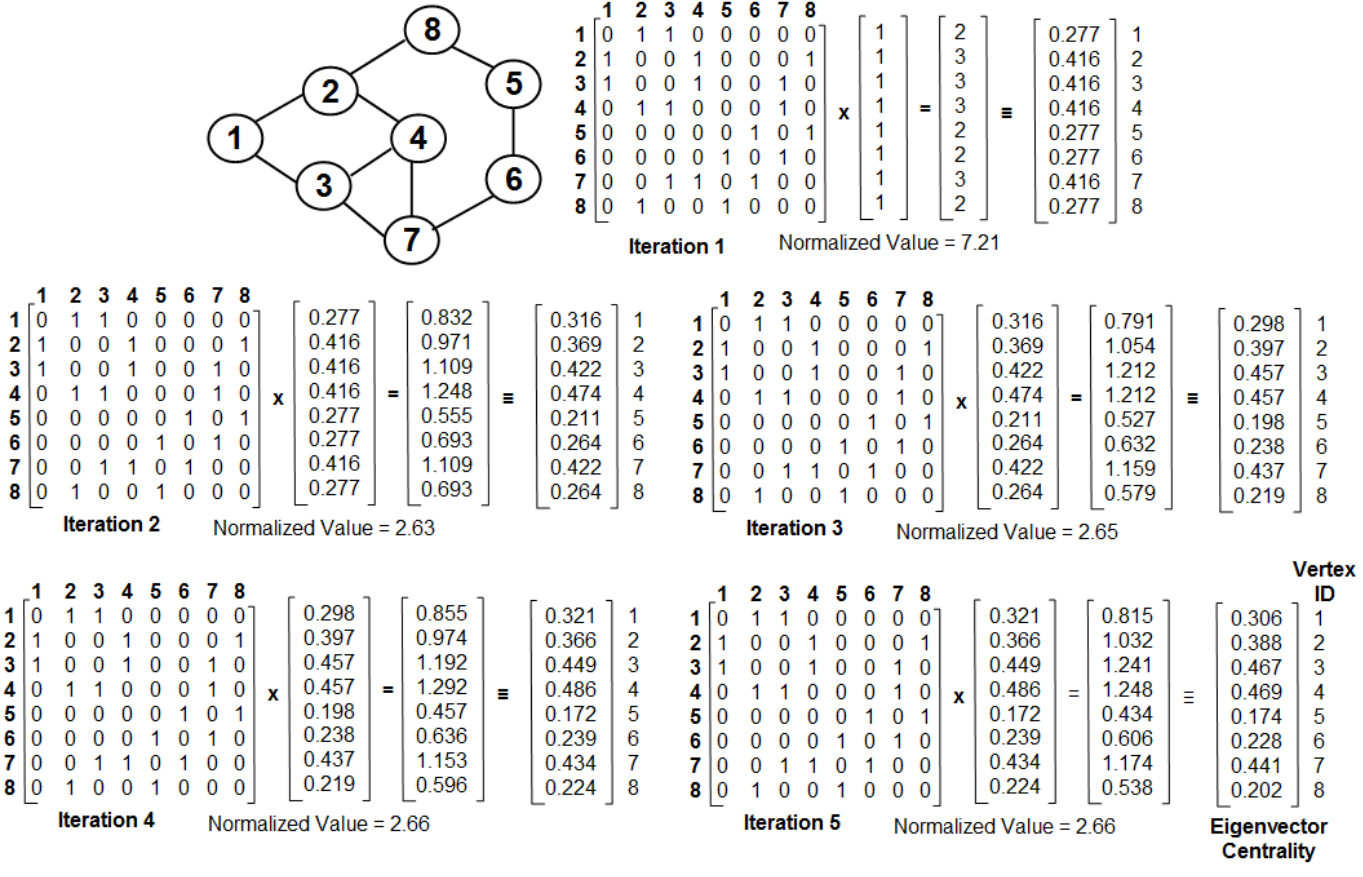
\includegraphics[scale=.32]{Abbildungen/eigenvektor_centrality_example.png}
	\caption[Eigenvektor Centrality: Power-iteration Method \cite{meghanathan_use_2015}]{Eigenvektor Centrality: Power-iteration Method \cite{meghanathan_use_2015}}
\end{figure}
Der limitierende Faktor dieser Methode zur Berechnung der "`Eigenvektor Centrality"' ist die Matrix-Multiplikation. Implementiert man diese naiv so ergibt sich eine Komplexität von \(O(n^3)\). Die Normierung lässt sich in linearer Laufzeit realisieren. Somit ist die Berechnung mit der "`Power-iteration method"' in polynominaler Laufzeit möglich. Die Metrik selbst lässt sich nativ in Wolfram und in Matlab finden. \cite{wolfram_graph_2020,matlab_measure_2020}
}
\subsubsection*{Page Rank}
{
Zum Abschluss der Zentralitätsmetriken soll eine Metrik dieser Kategorie vorgestellt werden, die einen hohen praktischen Nutzen findet. Der "`Page Rank"' oder die "`Page Rank Centrality"' beschreibt die Wichtigkeit eines Knotens auf Basis seines Ausgangsgrads, bzw. seiner Verbindungen zu anderen Knoten und des "`Page Ranks"' seiner benachbarten Knoten. Hierbei ähneln sich "`Page Rank"' und "`Eigenvektor Centrality"'. Die Metrik wurde erstmals in einem Google-Paper von Page und Brin veröffentlicht und soll Webseiten im World Wide Web bewerten. \cite{brin_anatomy_1998}

Es sei \(A\) eine Seite, bzw. ein Knoten und dieser Knoten hat Einwegkanten (Links) zu den Seiten \(T_1\dots T_n\). \(d\) sei ein frei wählbarer "`Dämpfungs"'-Faktor, der meist auf 0,85 gesetzt wird. Zudem ist \(C(A)\) als der Ausgangsgrad für eine Seite (Knoten) definiert. Der "`Page Rank"' ist dann folgendermaßen definiert.
\[
	PR(A) = (1-d)+d(\frac{PR(T_1)}{C(T_1)}+\dots +\frac{PR(T_n)}{C(T_n)})
\]
Die Berechnung des "`Page Ranks"' erfolgt durch einen iterativen Algorithmus, bie dem zunächst jedem Knoten der "`Page Rank"' \(1/|V|\) gegeben wird. Darauf aufbauend kann dann die obige Funktion zur weiteren Berechnung und die weiteren Iterationen herangenommen werden, bis die Metrik konvergiert. Der Algorithmus weißt dabei eine Zeit-Komplexität von \(O(k\cdot |E|)\) auf, wobei \(k\) für die Anzahl der Iterationen steht. \cite{oracle_pagerank_2017} "`Page Rank"' ist in allen angeführten Mathematikbibliotheken vertreten. \cite{sagemath_generic_nodate,wolfram_graph_2020,matlab_measure_2020}
}
\section{Chromatische Zahl und chromatischer Index}
{
Ein bekanntes Problem der Informatik ist das Färbeproblem. Es geht dabei darum einen Graphen so zu färben, sodass zwei benachbarte Knoten nicht die selbe Farbe haben. Anwendungen dafür kann man in vielen Problemen finden. Klassischerweise nimmt man das Beispiel der Karteneinfärbung bei der jedes Land ein Knoten ist und die Karte so eingefärbt werden soll, dass zwei benachbarte Länder nicht die gleiche Farbe haben. Allerdings lässt sich das Färbeproblem auch auf andere relevantere Probleme anwenden. Man kann z.B. so auch einen konfliktfreien Stundenplan erstellen oder andere ähnliche Konflikt-Probleme lösen. Die Eckenfärbung eines Graphen selbst ist eine Abbildung \(c: V\mapsto S\), wobei S die Menge an möglichen Färbungen ist. \cite{diestel_graphentheorie_2000,aigner_graphentheorie_2015} 
}
\subsubsection*{Chromatische Zahl}
{
Auf Basis der Färbeproblems können nun eine Reihe an Metriken definiert werden. Betrachtet man das Problem mithilfe der Abbildungsfunktion \(c\), so ist der Graph korrekt gefärbt, wenn gilt: \(\forall v, w (v\in V\land w\in V \land adjazent(v, w)\Rightarrow c(v)\neq c(w))\). Die "`chromatische Zahl"' beschreibt nun die Mächtigkeit der minimalen Menge \(S\) für die diese Bedingung zutrifft. Man bezeichnet die chromatische Zahl auch als \(\chi (G)\). Für einen leeren Graphen ist die chromatische Zahl 1. Liegt ein bipartiter Graph vor, so ist die chromatische Zahl offensichtlicherweise 2. \cite{diestel_graphentheorie_2000} Die chromatische Zahl kann sowohl von SageMath als auch von Wolfram berechnet werden \cite{sagemath_graph_2020-1,wolfram_wolfram_2020-1}

Das Herausfinden der chromatischen Zahl ist ein NP-vollständiges Problem und kann deshalb vermutlich auch nicht effizient berechnet werden. \cite{weisstein_chromatic_nodate,karp_reducibility_1996} So ist es möglich mittels eines Brute-Force-Algorithmus sämtliche Färbemöglichkeiten durchzuarbeiten und dann die Färbung herausnehmen, die gültig ist und die niedrigste Anzahl an Farben hat. Dieser Ansatz hätte eine exponentielle Laufzeit, die schon bei kleinen Graphen zu extrem hohen Rechenzeiten führen würde. Neben dieser naiven Variante werden u.a. auch heuristische Algorithmen genutzt, die versuchen die chromatische Zahl effizient zu approximieren. Ein bekannter Algorithmus hierfür ist folgendermaßen gegeben:
\begin{lstlisting}
	Chromatic-Number(G(V, E))
		vertices <- sortiere_nach_Grad_absteigend(V)
		highestColor <- 1
		for (vertex in vertices)
			color <- lowestPossibleColor(G, vertex)
			vertex.color = color
			highestColor <- Max{highestColor, color}
		return highestColor
\end{lstlisting}
Dieser Algorithmus hat allerdings den Nachteil, dass es nur eine Annäherung an die chromatische Zahl ist und nicht gesichert ist, dass das Ergebnis korrekt ist. Seine Strategie besteht darin, den Graphen mit möglichst wenig Farben zu färben, indem zuerst der Knoten gefärbt wird, der die meisten Nachbarn hat. 
}
\subsubsection*{Chromatischer Index}
{
Neben der Markierung bzw. Färbung von Knoten, ist es auch möglich in einem Graphen Kanten zu färben. Hierbei ist ähnlich wie bei der Knotenfärbung gemeint, dass eine Kante aus der Menge \(E(G)\) auf eine Zahl, bzw. Farbe abgebildet wird: \(k: E\mapsto S\). Im Rahmen der Kantenfärbung ist es nun wichtig, dass zwei indizente Kanten nicht die selbe Farbe zugewiesen bekommen. Das bedeutet, dass die Farben aller Kanten, die mit dem gleichen Knoten verbunden sind, alle eine unterschiedliche Farbe haben müssen. Formal lässt sich das so ausdrücken: \(\forall v,w(v\in E \land w\in E \land inzident(v,w)\Rightarrow k(v)\neq k(w))\). Findet man eine Abbildung, für die diese Bedingung zutrifft, so nennt man den Graphen \(k\)-Kanten-färbbar. \(k\) ist dabei die Mächtigkeit der Menge S, der gefundenen Abbildung. Das niedrigst mögliche \(k\) für einen Graphen ist dann dessen "`chromatischer Index"'. Man schreibt für dafür auch \(X'(G)\) Der "`chromatischer Index"' ist sowohl in Wolfram, als auch in SageMath verfügbar. \cite{andersen_edge-colorings_1977,sagemath_graph_2020-1,wolfram_wolfram_2020-1}

Jeder Graph fällt bei Betrachtung seines chromatisches Indexes in eine von zwei Klassen. Bei der ersten Klasse ist der chromatische Index \(X'(G)=\Delta(G)\), wobei \(\Delta(G)\) der Maximalgrad des Graphen ist. Fällt der Graph nicht in diese Klasse, so ist sein chromatischer Index \(X'(G)=\Delta(G)+1\). Obwohl dabei der chromatische Index sich pro Graph in einem extrem engen Korridor aufhält, ist die exakte Ermittlung des Indexes ein NP-vollständiges Problem und somit vermutlich nicht effizient, also in polynomialer Laufzeit, zu berechnen. Allerdings gibt es Spezialfälle, bei denen die Zuordnung des Graphen in einer der beiden Klassen einfach ist. So ist \(X'(G)=\Delta(G)\), wenn der Graph bipartit ist. Ist der Graph vollständig und die Anzahl der Knoten ist gerade, ist dies ebenfalls der Fall. Ein kompletter Graph mit ungerader Knotenanzahl hat dann logischerweise den chromatischen Index \(X'(G)=\Delta(G)+1\). \cite{plantholt_chromatic_1983}

Anwendung findet die Kantenfärbung in verschiedenen praktischen Problemen. Beispielsweise kann man es nutzen, um ein sogenanntes "`Round-Robin"'-Turnier mit möglichst wenig Runden zu planen. Ein "`Round-Robin"'-Turnier ist ein Turnier, bei dem jeder Teilnehmer auf jeden Teilnehmer einmal trifft. Dieses Problem ist zu lösen, indem jeder Teilnehmer durch einen Knoten repräsentiert wird und jede Begegnung durch eine Kante. Eine Farbe repräsentiert eine Runde. Werden die Kanten nun so gefärbt, dass der Turnier-Graph \(k\)-Kanten-gefärbt ist, hat man einen Turnier-Plan gefunden, der keine Konflikte hat. Ist der Graph zudem \(X'(G)\)-Kanten-gefärbt, so hat man den Plan gefunden, der möglichst wenig Runden erfordert. Der chromatische Index gibt in diesem Zusammenhang also an, wie viele Runden man minimal benötigt, sodass sich alle Teilnehmer einmal begegnen. Da der Graph bei dem sich alle einmal begegnen ein vollständiger Graph sein muss, ist auch schnell ersichtlich, wie viele Runden man braucht, betrachtet man die Ergebnisse des letzten Abschnitts. Neben "`Round-Robin"'-Turnieren lassen sich auch individuelle Turniere so planen. \cite{gross_handbook_2004}
}
\subsubsection*{Fraktionierte chromatische Zahl}
{
Neben der klassischen Art und Weise einen Graphen zu färben gibt es auch weitere Methoden. In der fraktionierten Graphentheorie ist es auch möglich in einem Graphen seinen Knoten mehrere Farben zuzuweisen. Auf Basis dessen lassen wich weitere Metriken definieren, die die Graphenfärbung als Grundlage haben. Hierzu zählt die "`fraktionierte chromatische Zahl"'. Um diese Zahl zu definierten, ist zunächst zu klären, wie fraktionierte Färbung formal definiert werden kann. Eine \(b\)-fache Färbung eines Graphen weist jedem Knoten eine Menge an \(b\) Farben zu. Auch dies kann durch eine Abbildung dargestellt werden, indem ein Knoten auf eine Menge an Färbungen abgebildet wird. Bei der Färbung muss nun darauf geachtet werden, dass zwei adjazente Knoten mit ihren zugewiesenen Farben keine Schnittmenge bilden. Besser kann dies durch eine Abbildung dargestellt werden. Sei \(A\) die Menge an verfügbaren Farben, so kann die Färbung mit folgender Abbildung dargestellt werden: \(c: V\mapsto A^b\). Für die Graphen-Färbung muss nun gelten: \(\forall v,w(v\in V\land w\in V\land adjazent(v,w)\Rightarrow c(v)\cap c(w)=\emptyset)\). Für eine \(b\)-Färbung wird eine bestimmte Anzahl \(a\) an Farben benötigt. Zu einer solchen Färbung wird dann auch gesagt, dass es eine \(a:b\)-Färbung ist. Das niedrigste \(a\) für das ein Graph eine \(b\)-Färbung hat, nennt man die \(b\)-fache chromatische Zahl (\(\chi _b(G)\)). Dabei ist logischerweise \(\chi_1(G) = \chi (G)\). Die fraktionierte chromatische Zahl ist dabei im Gegensatz folgendermaßen definiert \cite{scheinerman_fractional_2011}:
\[\chi_f(G)=\lim_{b\to\infty}\frac{\chi_b(G)}{b}\]
Die fraktionierte chromatische Zahl ist also der Grenzwert für die \(b\)-fache chromatische Zahl geteilt durch \(b\), wenn \(b\) gegen unendlich geht. Im Gegensatz zur "`normalen"' chromatischen Zahl ist die fraktionierte chromatische Zahl eine rationale und keine natürliche Zahl. Die Berechnung der Metrik ist ein NP-vollständiges Problem. Allerdings gibt es für einige Graphen vorgefertigte Werte, die genutzt werden können. So ist die fraktionierte chromatische Zahl eines zyklischen Graphen \(C_{2n+1}\) z.B. \(2+(\frac{1}{n})\). Der Algorithmus zur Berechnung der Kennzahl bedient sich einem linearem Programm und ist äußerst schwer zu berechnen. Die Komplexität steigt exponentiell zur Ordnung des Graphen. Eine native Implementierung dazu findet sich in SageMath. Wie bei der normalen Färbung kann auch die fraktionierte Färbung für diverse konfliktfreie Planungen und dergleichen verwendet werden. \cite{weisstein_chromatic_nodate,sagemath_graph_2020-1,scheinerman_fractional_2011}
}
%\subsubsection*{Fraktionierter chromatischer Index}
%{
%
%}
\section{Arborizität}
{
Ein wichtiger Teil der Graphentheorie ist die Betrachtung von Bäumen. Ein Baum ist dabei eine Zusammenhangskomponente eines Waldes. Ein Wald wiederum ist ein Graph, der keine Zyklen aufweist. Mithilfe dieses Wissens kann eine weitere Metrik definiert werden. Betrachtet man einen Graphen, zusammenhängend oder nicht, kann man sich die Frage stellen, wie es möglich ist, diesen Graphen aus einer Menge an Wäldern zu erstellen. Wichtiger noch ist es herauszufinden, aus welcher minimalen Anzahl an Wäldern es möglich ist, den vorliegenden Graphen aufzubauen. Diese minimale Anzahl ist die "`Arborizität"'. Präziser ausgedrückt, ist die "`Arborizität"' von \(G\) (\(Y(G)\)) die minimale Anzahl an azyklischen Subgraphen (Wäldern), dessen Vereinigung \(G\) ergibt. Hierbei teilen sich die Subgraphen keine gemeinsamen Kanten. \cite{weisstein_arboricity_nodate}

Zur Berechnung der Arborizität lassen sich sowohl Spezialfälle ausmachen, aber auch eine allgemeine Berechnungsvorschrift finden. So ist es zunächst ersichtlich, dass ein bereits azyklischer Graph eine Arborizität von \(Y(G)=1\) hat. Ein vollständiger Graph \(K_n\) hat wiederum eine Arborizität von \(Y(K_n)=\ceil[\big]{n:2}\) und ein vollständiger bipartiter Graph \(K_{m,n}\) weißt den Wert \(Y(K_{m,n})=\ceil[\big]{(mn):(m+n-1)}\) auf. Möchte man die Arborizität allgemein berechnen, ist ein bestimmter Parameter des Graphen zu berechnen. \(m_p\) gibt die maximale Anzahl an Kanten eines Subgraphen von \(G\) an, der \(p\) Knoten hat. Dieser Wert \(m_p\) muss nun für alle \(|G|>p>1\) berechnet werden. Mit dieser Berechnung lässt sich die Arborizität mit folgender Formel für jeden \(G\) ermitteln. \cite{weisstein_arboricity_nodate,nash-williams_edge-disjoint_1961}
\[Y(G)=\max_{p>1}\ceil[\Bigg]{\frac{m_p}{p-1}}\]
Die Berechnung der Arborizität ist in polynomialer Laufzeit möglich und kann in verschiedesten Szenarien angewandt werden. Einerseits kann es als Graph-Dichte-Maß herangezogen werden, da ein dichter, mit vielen Kanten durchzogener Graph, logischerweise eine höhere Arborizität aufweisen muss. Wie bereits in vorigen Kapiteln erwähnt, kann die Dichte für die Zuverlässigkeit bzw. Angriffssicherheit eines Netzwerks herangezogen werden. Weiterhin kann die Arborizität aber auch z.B. Aussagen über die Steifigkeit von Strukturen machen oder bei der Analyse von elektrischen Netzwerken helfen. Die Metrik ist in SageMath fest eingebaut. \cite{gabow_forests_1992,sagemath_graph_2020}

Die Spezialisierung der Arborizität ist die "`lineare Arborizität"'. Um diese Metrik zu definieren, muss zunächst der Begriff des "`linearen Waldes"' geklärt werden. Wie ein normaler Wald besteht ein linearer Wald ausschließlich aus azyklischen Graphen. Allerdings ist jede Zusammenhangskomponente des linearen Waldes ein Pfad. Man kann sich also einen linearen Wald graphisch als eine Ansammlung von vollständig unverzweigten Graphen vorstellen. Die "`lineare Arborizität"' \(la(G)\) ist nun analog zur normalen Arborizität die minimale Anzahl an linearen Wäldern, dessen Vereinigung \(G\) ergibt. \cite{alon_linear_1988}

Auch für die Berechnung dieser Metrik können Spezialfälle ausgemacht werden. Beispielsweise hat jeder \(d\)-reguläre Graph eine lineare Arborizität von \(\ceil[\big]{(d+1)/2}\). Außerdem konnte mithilfe des "`Linear Arboricity Conjecture"' bewiesen werden, dass für alle planaren Graphen gilt, dass die lineare Arborizität \(\ceil[\big]{\Delta :2}\) oder \(\ceil[\big]{(\Delta +1):2}\) ist. \(\Delta\) ist dabei der Maximalgrad von \(G\). Im Gegensatz zur normalen Arborizität ist die Ermittlung der linearen Arborizität nicht in polynomialer Laufzeit berechnenbar. Die Ermittlung dieser Metrik ist ein NP-vollständiges Problem. Die Kennzahl ist zudem in keiner er genannten Bibliotheken vorhanden. \cite{peroche_np-completeness_1984,calamoneri_planar_2010}
}
\section{Weitere Metriken}
{
Nachdem nun eine weite Reihe an Metriken vorgestellt wurde und diese jeweils in eine Kategorie eingeordnet wurden, sollen in diesem letzten Teil Graph-Kennzahlen vorgestellt werden, die nicht in eine der Kategorien passen aber dennoch Erwähnung finden sollen.
\subsubsection*{Unabhängigkeitszahl}
{
Bei der Betrachtung von Graphen ist es möglich sogenannte "`unabhängige"' Knotenmengen zu finden. Eine "`unabhängige"' Knotenmenge ist eine Untermenge \(S\) der Knoten \(V(G)\) (\(S\subseteq V(G)\)), sodass keiner der Knoten in \(S\) adjazent sind. Betrachtet man beispielsweise einen bipartiten Graphen, so ist ja dessen Definiton so gestaltet, dass der Graph in zwei "`unabhängige"' Knotenmengen gegliedert werden kann. Um nun die sogenannte "`Unabhängigkeitszahl' \(\alpha(G)\) für einen Graphen \(G\) zu ermitteln, muss man die größtmögliche "`unabhängige"' Knotenmenge für \(G\) finden. Die Mächtigkeit dieser Menge ist dann die "`Unabhängigkeitszahl"' von \(G\) \cite{diestel_graphentheorie_2000,weisstein_maximum_nodate,weisstein_maximum_nodate} Unterstützung für diese Metrik lässt sich SageMath und Wolfram direkt oder indirekt (Ausgabe der größten "`unabhängigen"' Knotenmenge) finden. \cite{sagemath_graph_2020,weisstein_independence_nodate}

Die Berechnung der "`Unabhängigkeitszahl"' erfolgt durch das finden der größten "`unabhängigen"' Knotenmenge. Dieses Problem ist NP-schwer und lässt sich durch einen navien Brute-Force-Algorithmus lösen. Dieser iteriert über jedes mögliche Subset von \(G\) und prüft, ob das Subset unabhängig ist. Ist über alle Untermengen iteriert worden, kann die Mächtigkeit der größten, unabhängigen Untermenge ermittelten werden. Die Zahl der zu untersuchenden Untermengen steigt exponentiell mit jedem weiteren Knoten. Durch Optimierungen und intelligente Algrotihmen kann das Problem mittlerweile in einer Zeitkomplexität von \(O(1,1996^n)\) gelöst werden. \cite{xiao_exact_2017}
}
\subsubsection*{Cliquenzahl}
{
Verwandt mit der Unabhängigkeitszahl ist die sogenannte "`Cliquenzahl"'. Wenn von Cliquen bei Graphen die Rede ist, ist eine Untermenge in einem Graphen \(G\) gemeint, in der jeder Knoten adjazent ist zu jedem anderen Knoten innerhalb der Untermenge. Deutlicher kann man es so ausdrücken, dass eine Clique in einem Graphen eine Untermenge an Knoten ist, die gemeinsam einen vollständigen Graphen bilden. Die Cliquenzahl \(\omega(G)\) ist nun die größte Mächtigkeit einer Knotenmenge, die in G eine Clique formt. \cite{diestel_graphentheorie_2000} Auch die Cliquenzahl lässt sich in Wolfram und in SageMath finden \cite{wolfram_research_findclique_2015,sagemath_graph_2020} Das auffinden von Cliquen ("`Cliquenproblem"') und damit auch das ermitteln der Cliquenzahl ist ein NP-vollständiges Problem und kann deshalb vermutlich auch nicht effizient gelöst werden.

Das Prinzip der Clique kann, wie der Name schon nahelegt, beispielsweise auf sozialen Netze übertragen werden. Stellen Knoten Personen dar und Kanten Freundschaften, können durch das Auffinden von Graph-Cliquen echte Personen-Cliquen gefunden werden. Die Cliquenzahl eines Graphen gäbe in diesem Kontext dann Größe der größten Clique innerhalb eines sozialen Netzes an.
}
\subsubsection*{Buchdicke/Seitenzahl}
{
Als letztes soll noch eine geometrische Invariante untersucht und beschrieben werden: Die "`Buchdicke"' bzw. "`Seitenzahl"' \(bt(G)\) eines Graphen \(G\). Hierfür muss zunächst geklärt werden, was ein "`Buch"' im Rahmen der Graphentheorie ist. Ein \(n\)-Buch, bzw. ein "`Buch"' mit \(n\) Seiten besteht aus einer Linie ("`spine"' oder "`Rücken"') \(L\), die sich in einem dreidimensionalen Raum aufhält und \(n\) Halb-Ebenen ("`Seiten"'), die L als ihre gemeinsame Grenze haben, an denen sie sich treffen. Ein ein solches Buch kann man nun einen Graphen hineinlegen. Hierbei liegt jeder Knoten auf dem "`Buchrücken"' \(L\) und jede Kante liegt auf einer der "`Seiten"'. Hierbei ist es wichtig, dass sich die Kanten auf einer Seite nicht kreuzen drüfen. Um dies besser zu verdeutlichen, wie sich dies graphisch wiederspiegelt sei Abbildung 2.2 gegeben. Gezeigt wird wie ein vollständiger Graph mit fünf Knoten in ein Buch eingebettet wird.
\begin{figure}[ht!]
	\centering
	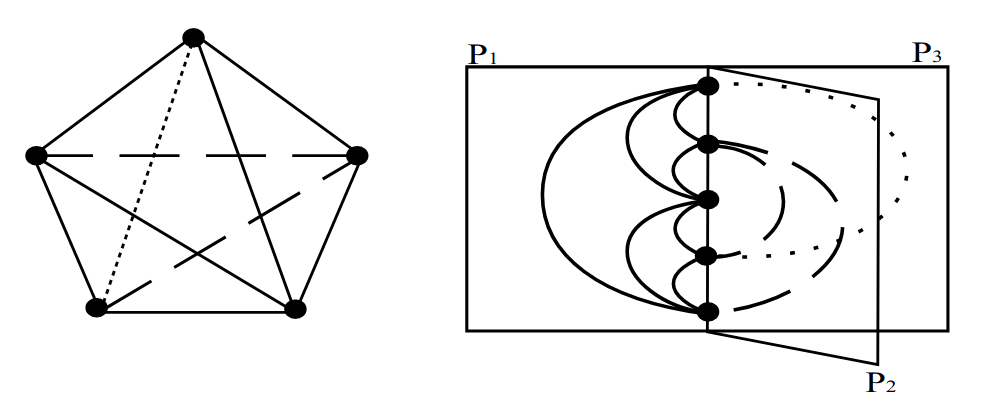
\includegraphics[scale=0.4]{Abbildungen/graph_book.png}
	\caption[Einbettung \(K_5\) in Buch \cite{blankenship_book_2003}]{Einbettung \(K_5\) in Buch \cite{blankenship_book_2003}}
\end{figure}
Die "`Buchdicke"' bzw. "`Seitenzahl"' \(bt(G)\) ist nun das kleinsmögliche \(n\) das gefunden werden kann, damit der Graph in das korrespondierende \(n\)-Buch hineingelegt werden kann. \cite{bernhart_book_1979} Die ermittlung von \(bt(G)\), bzw. das Entscheidungsproblem, ob ein Graph \(G\) in ein \(n\)-Buch eingebettet werden kann, ist ein NP-vollständiges Problem. \cite{chung_embedding_1987}

Die "`Buchdicke"' und das Einbetten von Graphen in ein "`Buch"' hat mehrere Anwendungsszenarien. Eines davon ist die Planung einer Ampelschaltung einer Kreuzung. Hierbei betrachten wir die Knoten eines Graphen als die ein- und ausgehenden Straßenspuren (inkl. Fuß- und Radwege). Die Kanten sind die möglichen Wege, die ich von einem Knoten zum anderen begehen/befahren kann. Die Knoten sind nun so auf dem "`Buchrücken"' zu arrangieren, dass ihre Reihenfolge auf dem "`Rücken"' der Reihenfolge der Spuren im Uhrzeigersinn auf der Kreuzung gleicht. Die Kanten werden anschließend in die "`Seiten"' eingebettet. Jede "`Seiten"' repräsentiert dann eine Ampelphase, die so geschaltet ist, dass die Verbindungen der jeweiligen Seite befahrbar sind, ohne das es zu Konflikten kommt. Die "`Buchdicke"' ist infolgedessen auch die minimal mögliche Anzahl an Ampelphasen an einer gegeben Kreuzung \cite{kainen_book_1990}
}
\section{Übersicht der vorgestellten Graphmetriken}
{
Nachdem nun eine weite Reihe an Graph-Metriken vorgestellt wurden, sollen diese mit Hilfe einer Aufzählung zusammengefasst werden. Aufgelistet werden jeweils der Name, bzw die Bezeichnung, der Metrik und ihre Definition. Zudem soll klar werden in welche der Kategorien die Metrik gehört Bei der Definition wird dabei eine mathematische oder eine wörtliche Beschreibung angegeben. Gegebenenfalls auch beides, falls es für das Verständnis förderlich ist.

\metric{Ordnung \(|V(G)|\)}{Anzahl der Knoten eines Graphen}
\metric{Größe \(|V(E)|\)}{Anzahl der Kanten eines Graphen}
\metric{Knotengrad \(d(v)\)}{Anzahl der inzidenten Kanten des Knotens \(v\)}
\metric{Minimal- (\(\delta(G)\)) und Maximalgrad (\(\Delta(G)\))}{Der kleinste bzw. größte Knotengrads des Graphen \(G\); \(\delta (G):=min\{d(v)\ \vert\ v\ \in\ V(G)\}\), \(\Delta (G)\ :=\ max\{d(v)\ \vert\ v\ \in\ V(G)\}\)}
\metric{Anzahl der Zusammenhangskomponenten}{Anazahl der Komponenten/Subgraphen eines Graphen, die selbst zusammenhängend sind. Ein Graph (eine Komponente) ist dann zusammehängend, wenn sich zwischen zwei beliebigen seiner Knoten immer ein Weg finden lässt.}
\metric{Abstand/Distanz \(d_G(x,y)\)}{Die Länge des kürzesten Weges zwischen den beiden Knoten \(x\) und \(y\).}
\metric{Extrenzität eines Knotens \(ecc(x,G)\)}{Der Maximale Abstand, den ein Knoten zu einem anderen Knoten im Graphen \(G\) haben kann. \(ecc(x, G)=\max_{y\in V(G)}\{d_G(x,y)\}\)}
\metric{Durchmesser}{Der größte Abstand zweier Knoten innerhalb des Graphen \(G\). \(Durchmesser(G)=\max_{x,y}\{ d_G (x,y)\}\).}
\metric{Radius}{Kleinste Extrenzität innerhalb des Graphen. Extrenzität der Knoten des Zentrums. \(rad(G) = \min_{x\in V(G)}\max_{y\in V(G)}d_G(x,y)\).}
\metric{Taillenweite}{Länge des kürzesten Kreises innerhalb eines Graphen}
\metric{Umfang}{Länge des größten Kreises innerhalb eines Graphen}
\metric{Dichte}{Anzahl der Kanten des Graphen geteilt durch die Anzahl der möglichen Kanten. Ungerichteter Graph: \(\frac{\vert E\vert}{\binom{\vert V\vert}{2}}\). Gerichteter Graph: \(\frac{\vert E\vert}{2\binom{\vert V\vert}{2}}\)}
\metric{Stärke \(\sigma(G)\)}{Das Minimale Verhältnis zwischen entfernten Kanten und dadurch entstandenen Zusammenhangskomponenten. Sei \(\Pi\) die Menge aller möglichen Partitionierungen der Knoten \(V\) und \(\partial\pi\) die Menge an Kanten, die entfernt werden müssten, um die Partitionierung \(\pi\) zu erreichen, gilt folgende Formel zur Errechnung der Stärke:
\[\sigma(G)=\min_{\pi\in\Pi}\frac{\vert\partial\pi\vert}{\vert\pi\vert -1}\]}
\metric{"`Vertex Connectivity"'}{Minimale Anzahl \(k\) Knoten, die aus einem zusammenhängenden Graphen entfernt werden müssen, sodass er nicht mehr zusammenhängend ist.}
\metric{"`Edge Connectivity"'}{Minimale Anzahl \(k\) Kanten, die aus einem zusammenhängenden Graphen entfernt werden müssen, sodass er nicht mehr zusammenhängend ist.}
\metric{Degree Centrality}{Der Grad eines Knoten: \(d(v); v\in V\)}
\metric{Betweenness Centrality \(C_B(v)\)}{Wichtigkeitsmaß für einen Knoten, das angibt inwieweit beliebige kürzeste Wege zwischen zwei anderen Knoten durch ihn verlaufen. Sei \(\sigma_{st}\) Anzahl der kürzesten Wege zwischen Knoten \(s\) und \(t\) und \(\sigma_{st}(v)\) die Anzahl dieser Wege, die durch \(v\) laufen.
\[
	C_B(v)=\sum_{s\neq v\neq t\in V}\frac{\sigma_{st}(v)}{\sigma_{st}}
\]
}
\metric{Closeness Centrality \(C_C(v)\)}{Zentralitätsmetrik, die Knoten danach bewertet wie weit sie von jedem Anderen Knoten entfernt sind.
\[
	C_C(v)=\frac{|V|-1}{\sum_{u\in V}d_G(v,u)}	
\]
}
\metric{Eigenvektor Centrality \(x_v\)}{Zentralitätsmetrik, die einen Knoten dahingehend bewertet wie vernetzt er ist und wie vernetzt seine Nachbarn sind. Wendet man die Metrik auf die gesamte Adjazenzmatrix \(A\) an, so sind die Eigenvektor Centralities aller Knoten im Eigenvektor \(x\) zu finden, der nur positive Werte enthält.
\[
	x_v=\frac{1}{\lambda}\sum_{t\in M(v)}x_t=\frac{1}{\lambda}\sum_{t\in G}a_{v,t}x_t
\]
}
\metric{Page Rank}{Praktisch angewandte Zentralitätsmetrik, die ähnlich wie die Eigenvektor Centrality einen Knoten nach seiner v+Vernetztheit und der Vernetztheit seiner Nachbarn bewertet. Sei \(A\) der zu untersuchende Knoten (Seite) und \(T_1\dots T_n\) die Knoten auf die von \(A\) aus gezeigt wird (Links), dass ist der Page Rank PR(A) so definiert:
\[
	PR(A) = (1-d)+d(\frac{PR(T_1)}{C(T_1)}+\dots +\frac{PR(T_n)}{C(T_n)})
\]
}
}
\chapter{Ähnlichkeit von Graphen}

\chapter{Implementierung und Umsetzung der Metriken}

\section{Implementierung in verschiedenen Graphdatenbanken}

\section{Vergleich der Implementierungen}

\chapter{Graphmetriken und Ähnlichkeit in Anwendung}

\chapter{Fazit und Zusammenfassung}

\section{Zusammenfassung der Ergebnisse}

\section{Fazit}

\chapter*{Glossar}
\addcontentsline{toc}{chapter}{Glossar}
{
}
\printbibliography
\end{document}